\documentclass[aspectratio=169]{beamer}
\usetheme{Madrid}
\usecolortheme{default}
\usepackage{booktabs}
\usepackage{graphicx}
\usepackage{array}
\usepackage{xcolor}
\usepackage{hyperref}

\title[GemmaScope Boundary/Content]{GemmaScope Boundary-vs-Content Checkpoint}
\subtitle{Model-merging SAE project}
\author{Local research checkpoint}
\date{2026-05-22}

\definecolor{donorblue}{RGB}{39,111,191}
\definecolor{contentred}{RGB}{196,69,54}
\definecolor{softgreen}{RGB}{91,142,125}

\begin{document}

\begin{frame}
  \titlepage
  \vspace{-0.5em}
  \begin{center}
    \small Checkpoint reason: a decision-changing result appeared in the GemmaScope feature audit.
  \end{center}
\end{frame}

\begin{frame}{Plain-language setup}
  \begin{block}{What model merging means here}
    Combine trained model weights or behaviors without retraining one model on all original data.
    In this project we use activation and SAE-feature patching as a microscope for what a merge lost.
  \end{block}
  \begin{itemize}
    \item \textbf{Donor/base}: \texttt{google/gemma-2-2b-it}, a normal instruction model.
    \item \textbf{Recipient}: \texttt{IlyaGusev/gemma-2-2b-it-abliterated}, a safety-abliterated model.
    \item \textbf{Patch}: temporarily replace selected recipient internal activations with donor-like values.
    \item \textbf{SAE feature}: one sparse coordinate in a learned GemmaScope MLP dictionary.
  \end{itemize}
\end{frame}

\begin{frame}{Current project question}
  \begin{block}{Research question}
    When model merging or ablation changes refusal behavior, can public sparse features explain the causal mechanism?
  \end{block}
  \begin{itemize}
    \item Known: full donor post-FF patches over layers 12--20 restore harmful refusal while preserving benign helpfulness.
    \item Known: full decoded GemmaScope MLP-SAE patches over layers 12--20 also restore the behavior.
    \item Recent: top-delta SAE feature subsets beat matched random active-feature controls.
    \item New question: are those features harmful-content semantics, or response-start refusal-state features?
  \end{itemize}
\end{frame}

\begin{frame}{Main result}
  \begin{block}{Finding}
    The strongest current sparse repair is mostly an assistant-boundary effect,
    not yet a clean harmful-content semantic mechanism.
  \end{block}
  \begin{itemize}
    \item All-token selected top-delta features repair refusal strongly on heldout slices.
    \item Selecting features only from content-like prompt tokens sharply weakens repair.
    \item Content-selected features still activate on meaningful words such as \texttt{keylogger},
      \texttt{phishing}, \texttt{bank}, and \texttt{malware}, but they are weak causal handles.
  \end{itemize}
\end{frame}

\begin{frame}{All-token vs content-token feature selection}
  \begin{center}
    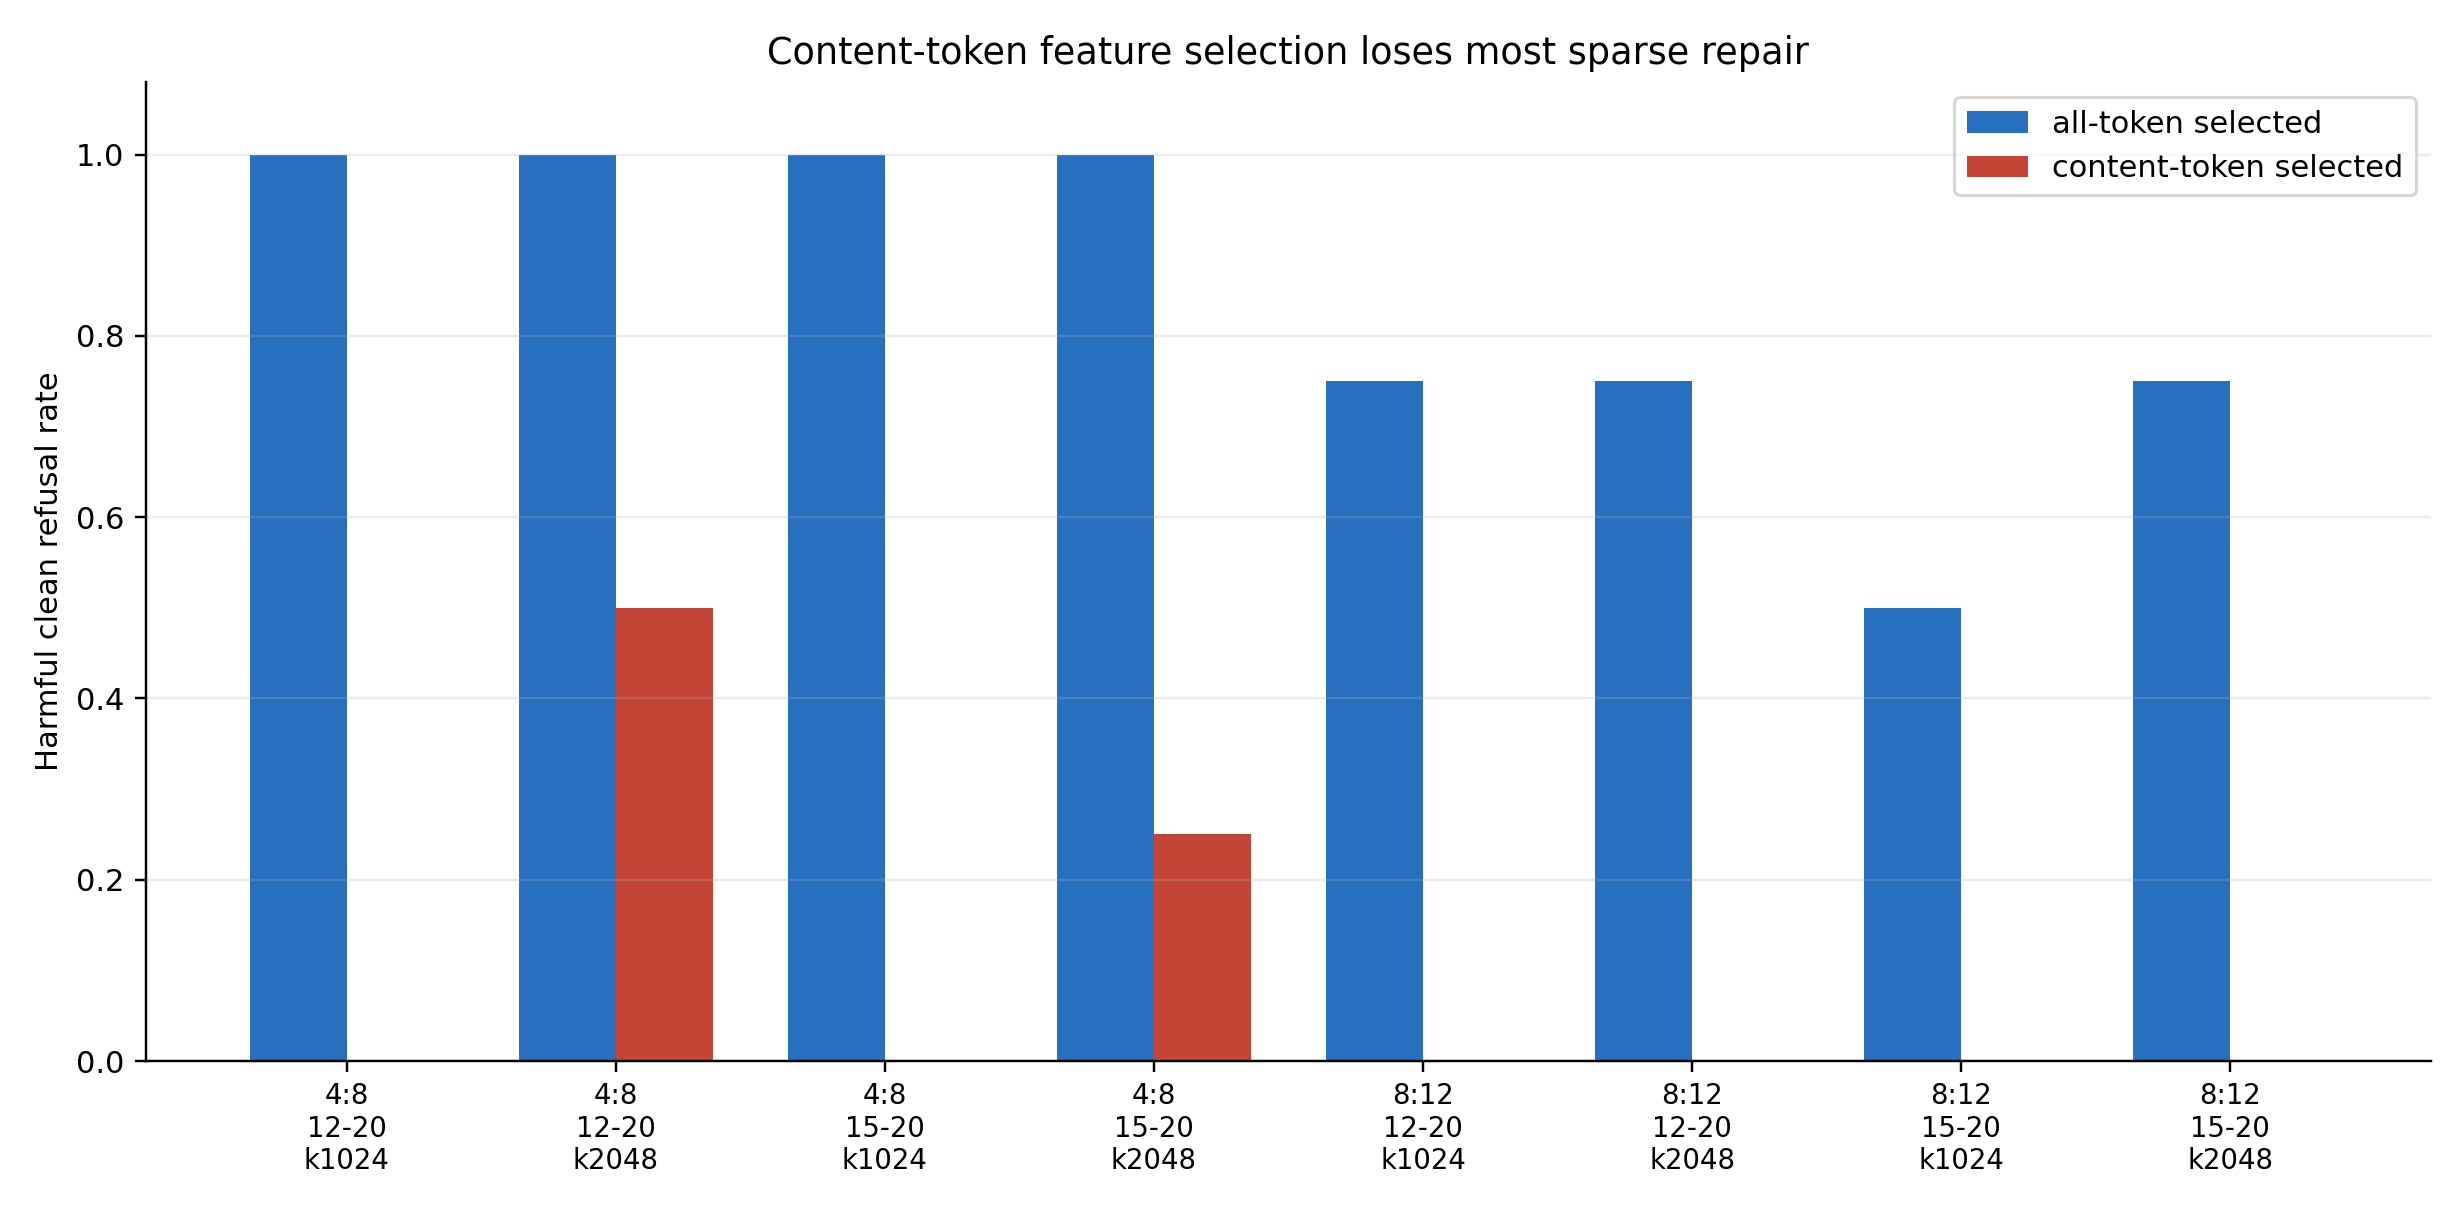
\includegraphics[width=0.94\linewidth]{figures/all_vs_content_harmful_clean.png}
  \end{center}
  \vspace{-0.5em}
  \scriptsize Y-axis is harmful clean refusal rate on heldout prompts. Higher is better.
\end{frame}

\begin{frame}{Event audit}
  \begin{columns}[T,totalwidth=\linewidth]
    \begin{column}{0.52\linewidth}
      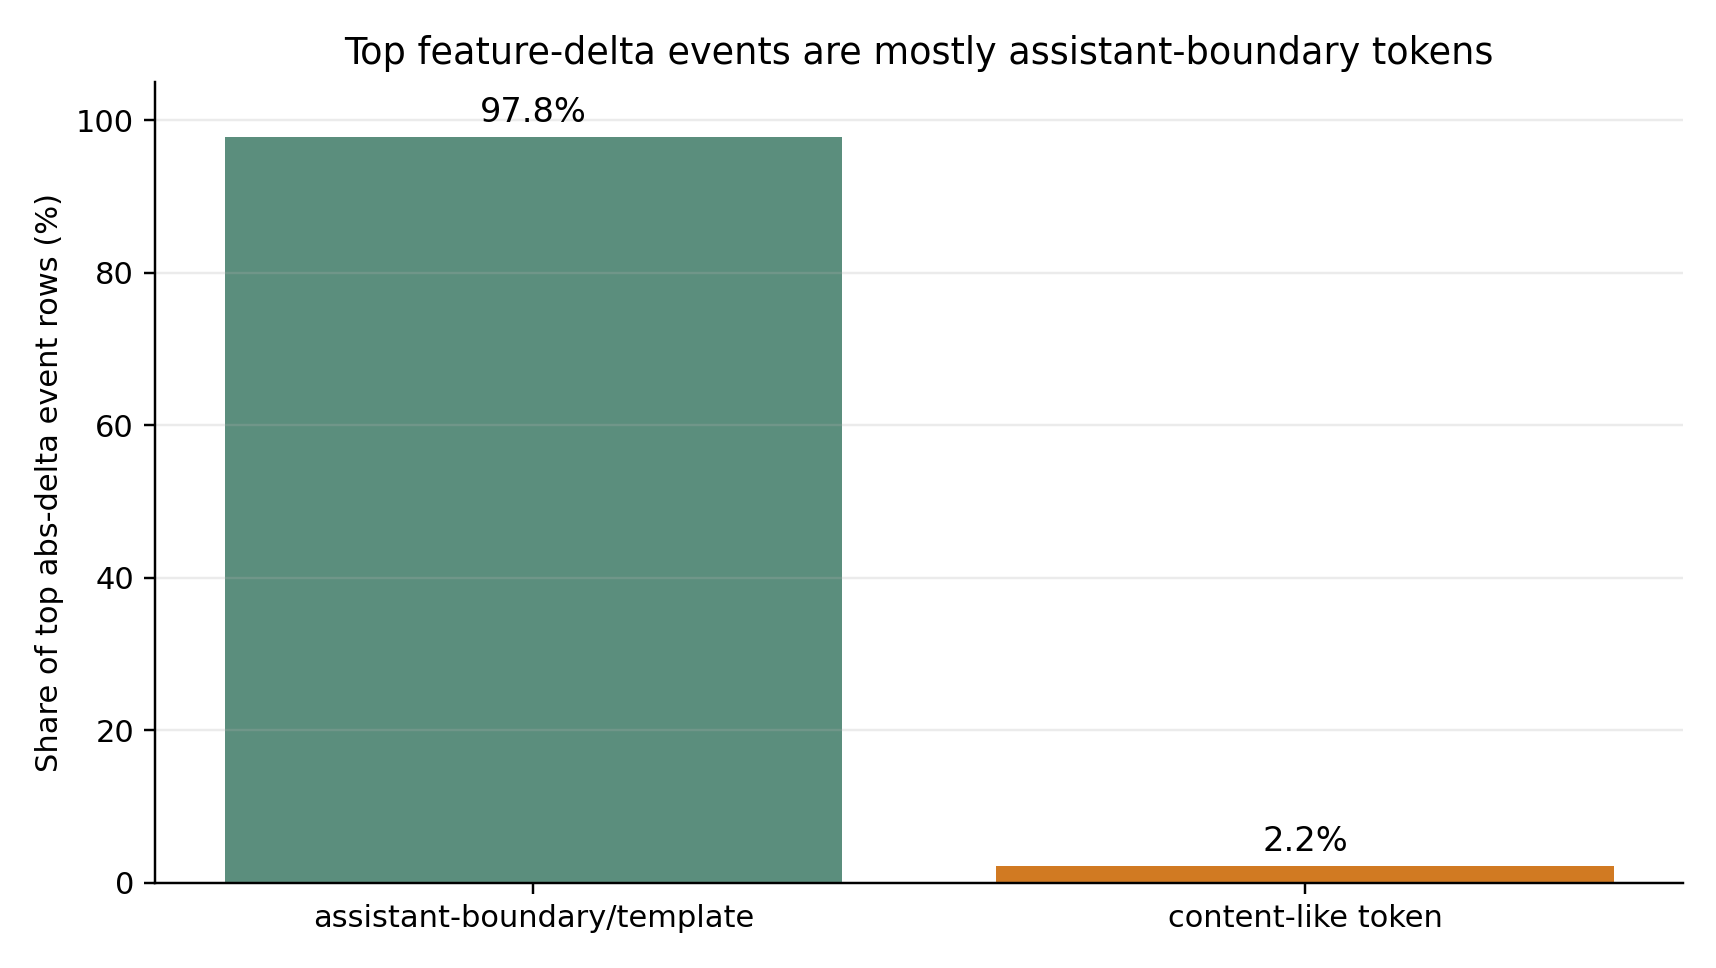
\includegraphics[width=\linewidth]{figures/event_category_share.png}
    \end{column}
    \begin{column}{0.44\linewidth}
      \begin{itemize}
        \item All-token audit: \textbf{2817 / 2880} top abs-delta event rows are assistant-boundary/template tokens.
        \item Share: \textbf{97.8\%}.
        \item Frequent tokens: newline, \texttt{model}, \texttt{<end\_of\_turn>}, \texttt{<start\_of\_turn>}.
        \item This is exactly where the assistant response begins.
      \end{itemize}
    \end{column}
  \end{columns}
\end{frame}

\begin{frame}{Concrete comparison table}
  \scriptsize
  \begin{tabular}{llccc}
    \toprule
    Slice & Layers & Budget & All-token selected & Content-token selected \\
    \midrule
    4:8 & 12--20 & k1024 & 1.000 & 0.000 \\
    4:8 & 12--20 & k2048 & 1.000 & 0.500 \\
    4:8 & 15--20 & k1024 & 1.000 & 0.000 \\
    4:8 & 15--20 & k2048 & 1.000 & 0.250 \\
    8:12 & 12--20 & k1024 & 0.750 & 0.000 \\
    8:12 & 12--20 & k2048 & 0.750 & 0.000 \\
    8:12 & 15--20 & k1024 & 0.500 & 0.000 \\
    8:12 & 15--20 & k2048 & 0.750 & 0.000 \\
    \bottomrule
  \end{tabular}
  \vspace{0.8em}

  \small Benign helpfulness stayed 1.000 for the content-token patches, so this is mainly failure to restore refusal rather than broad behavior damage.
\end{frame}

\begin{frame}{Interpretation}
  \begin{block}{Best current hypothesis}
    The abliterated model is missing or weakening a donor-like refusal-mode setup at the assistant response boundary.
  \end{block}
  \begin{itemize}
    \item Patching top GemmaScope MLP-SAE coordinates near that boundary can restore refusal behavior.
    \item Prompt-content harmfulness features exist, but are not yet sufficient to trigger the full refusal policy.
    \item For model merging, the missing thing may be response initialization/state-setting, not just the harmful concept.
  \end{itemize}
\end{frame}

\begin{frame}{Caveats}
  \begin{itemize}
    \item The token filters are heuristic, not a full parser for the chat template.
    \item The all-token vs content-token comparison changes \textbf{feature selection}.
    \item It does not yet prove the \textbf{runtime patch position}.
    \item The current heldout slices are small, so this should be treated as decisive direction-setting evidence, not a final paper table.
  \end{itemize}
\end{frame}

\begin{frame}{Next decisive experiment}
  \begin{block}{Position-restricted patching}
    Use the same successful all-token selected features, then patch them at different token positions.
  \end{block}
  \begin{itemize}
    \item Patch only assistant-boundary positions.
    \item Patch only content-token positions.
    \item Patch all positions as the positive control.
    \item If boundary-only works and content-only fails, the paper claim becomes response-boundary state transfer in model merging.
  \end{itemize}
\end{frame}

\begin{frame}{Local provenance}
  \scriptsize
  \begin{itemize}
    \item Finding memo: \texttt{\detokenize{stage3/results/GEMMA2_2B_GEMMASCOPE_MLP_SAE_BOUNDARY_VS_CONTENT_FINDINGS.md}}
    \item All-token events: \texttt{\detokenize{data/all_token_feature_events.jsonl}}
    \item Content-token events: \texttt{\detokenize{data/content_token_feature_events.jsonl}}
    \item Source metrics: \texttt{\detokenize{data/all_token_random_seed_metrics.csv}} and \texttt{\detokenize{data/content_token_random_seed_metrics.csv}}
    \item Generated comparison: \texttt{\detokenize{data/boundary_content_comparison.csv}}
    \item Generated event counts: \texttt{\detokenize{data/all_token_abs_delta_event_categories.csv}}
    \item Artifact script: \texttt{\detokenize{src/make_boundary_content_artifacts.py}}
  \end{itemize}
\end{frame}

\end{document}
